%!TEX root = ../main.tex
\section{Symphony: Reasoning over Multimodal Data Lakes}
\label{sec:reasoning}



In this section, we present the reasoning process of \sys, which integrates Large Language Models (LLMs) with Retrieval-Augmented Generation (RAG) to reason over information from multimodal data lakes. Given a natural language (NL) question, \sys first retrieves top-$k$ relevant data items from the data lakes, as discussed in the previous section. 
%
\sys then conducts a question decomposition strategy to address complex queries effectively, where a question can be decomposed into sub-questions, and each sub-question can be answered by different tools, such as LLMs, DBMSs, and so on. 

%Next, we explain how RAG, combined with an LLM, utilizes the retrieved data items to generate responses, including our method for aggregating answers across sub-questions. Finally, we outline optimization strategies designed to enhance both reasoning efficiency and accuracy.


\subsection{Question Decomposition}

We propose a Question Decomposition strategy to address complex questions requiring information from multiple sources. Here, a \textit{data source} is defined as a collection of data items originating from the same origin, such as an isolated table, a database, or a text passage. When multiple data items, like a table and passage, come from the same Wikipedia page or structured document, they are also treated as a single data source. Similarly, if two tables \(d_i\) and \(d_j\) have a predefined primary-foreign key (PK-FK) relationship, as with tables from the same database, they are merged into a unified data source \(d_k'\). Initially, we retrieve a set of data items \(D = \{d_1, d_2, \ldots, d_n\}\) from multimodal data lakes and process them using heuristic methods to form \(D' = \{d_1', d_2', \ldots, d_m'\}\), where $m \leq n$ and each \(d_i \in D'\) represents a distinct data source.

The \textbf{objective} of our question decomposition strategy is to break down a complex query into simpler sub-questions to facilitate retrieval of relevant information. Ideally, each sub-question should focus on a primary data source. However, we allow flexibility for sub-questions that still require multiple sources after decomposition, accommodating scenarios where information from different sources complements or corroborates each other. This adaptable approach enhances reasoning effectiveness by balancing simplicity, which reduces each sub-question to its essential elements, with the integration of supportive data, enabling relevant details from multiple sources to strengthen the answer's accuracy. Together, these elements minimize fusion errors and streamline the reasoning flow, creating a coherent, step-by-step resolution.

% The objective of question decomposition is to break down a complex question requiring multiple data sources into simpler sub-questions, ensuring that each sub-question can be answered using at most one data source. When only one data source is involved, decomposition is unnecessary. This approach enhances reasoning effectiveness by allowing each sub-question to focus on a single, relevant data source, minimizing potential errors from data fusion and simplifying the reasoning process. It also maintains a logical execution order, with each sub-question building on information gathered from previous ones, which strengthens coherence and accuracy across steps.

To achieve this, \sys employs an iterative prompt-based approach with LLM to automate the decomposition process. In each round, the LLM generates a sub-question based on the previous sub-question and data source, or decides to terminate the process. 
%
First, an initial prompt is generated to identify the first sub-question and its corresponding data sources. \sys then iteratively uses this information to generate subsequent prompts, guiding the LLM to create the next sub-question until the entire question is resolved. In cases where the LLM determines that a question cannot be effectively decomposed, \sys bypasses decomposition. Instead, it directly leverages the information retrieved from multiple data sources to formulate a reasoning for the original question. For example, a question like ``What is the population of France?'' cannot be further decomposed into distinct sub-questions.

%\begin{example}
We illustrate the question decomposition process in Figure~\ref{fig:reasoning}. Suppose we have a question {\bf Q}: ``Which song ...,'' with two relevant data sources retrieved from multimodal data lakes, a passage {\bf P1} and a table {\bf T1}.   Using a template-based approach, \sys constructs an initial prompt, $\mathbf{prompt}_0$, based on {\bf Q}, $P1$, and $T1$. \sys sends the prompt $\mathbf{prompt}_0$ to LLM, and LLM generate a sub-question {\bf q1} as well as the data source on which it should be utilized. Building on the first sub-question {\bf q1} and its data source {\bf P1}, \sys uses the next prompt template to generate $\mathbf{prompt}_1$. Given $\mathbf{prompt}_1$, the LLM generates the second sub-question, {\bf q2}, and assigns table {\bf T1} as its data source. 
At this point, the LLM decides to stop, as it considers the original query $Q$ fully addressed.
%\end{example}

\begin{figure}[t!]
%\vspace{-1em}
\begin{center}
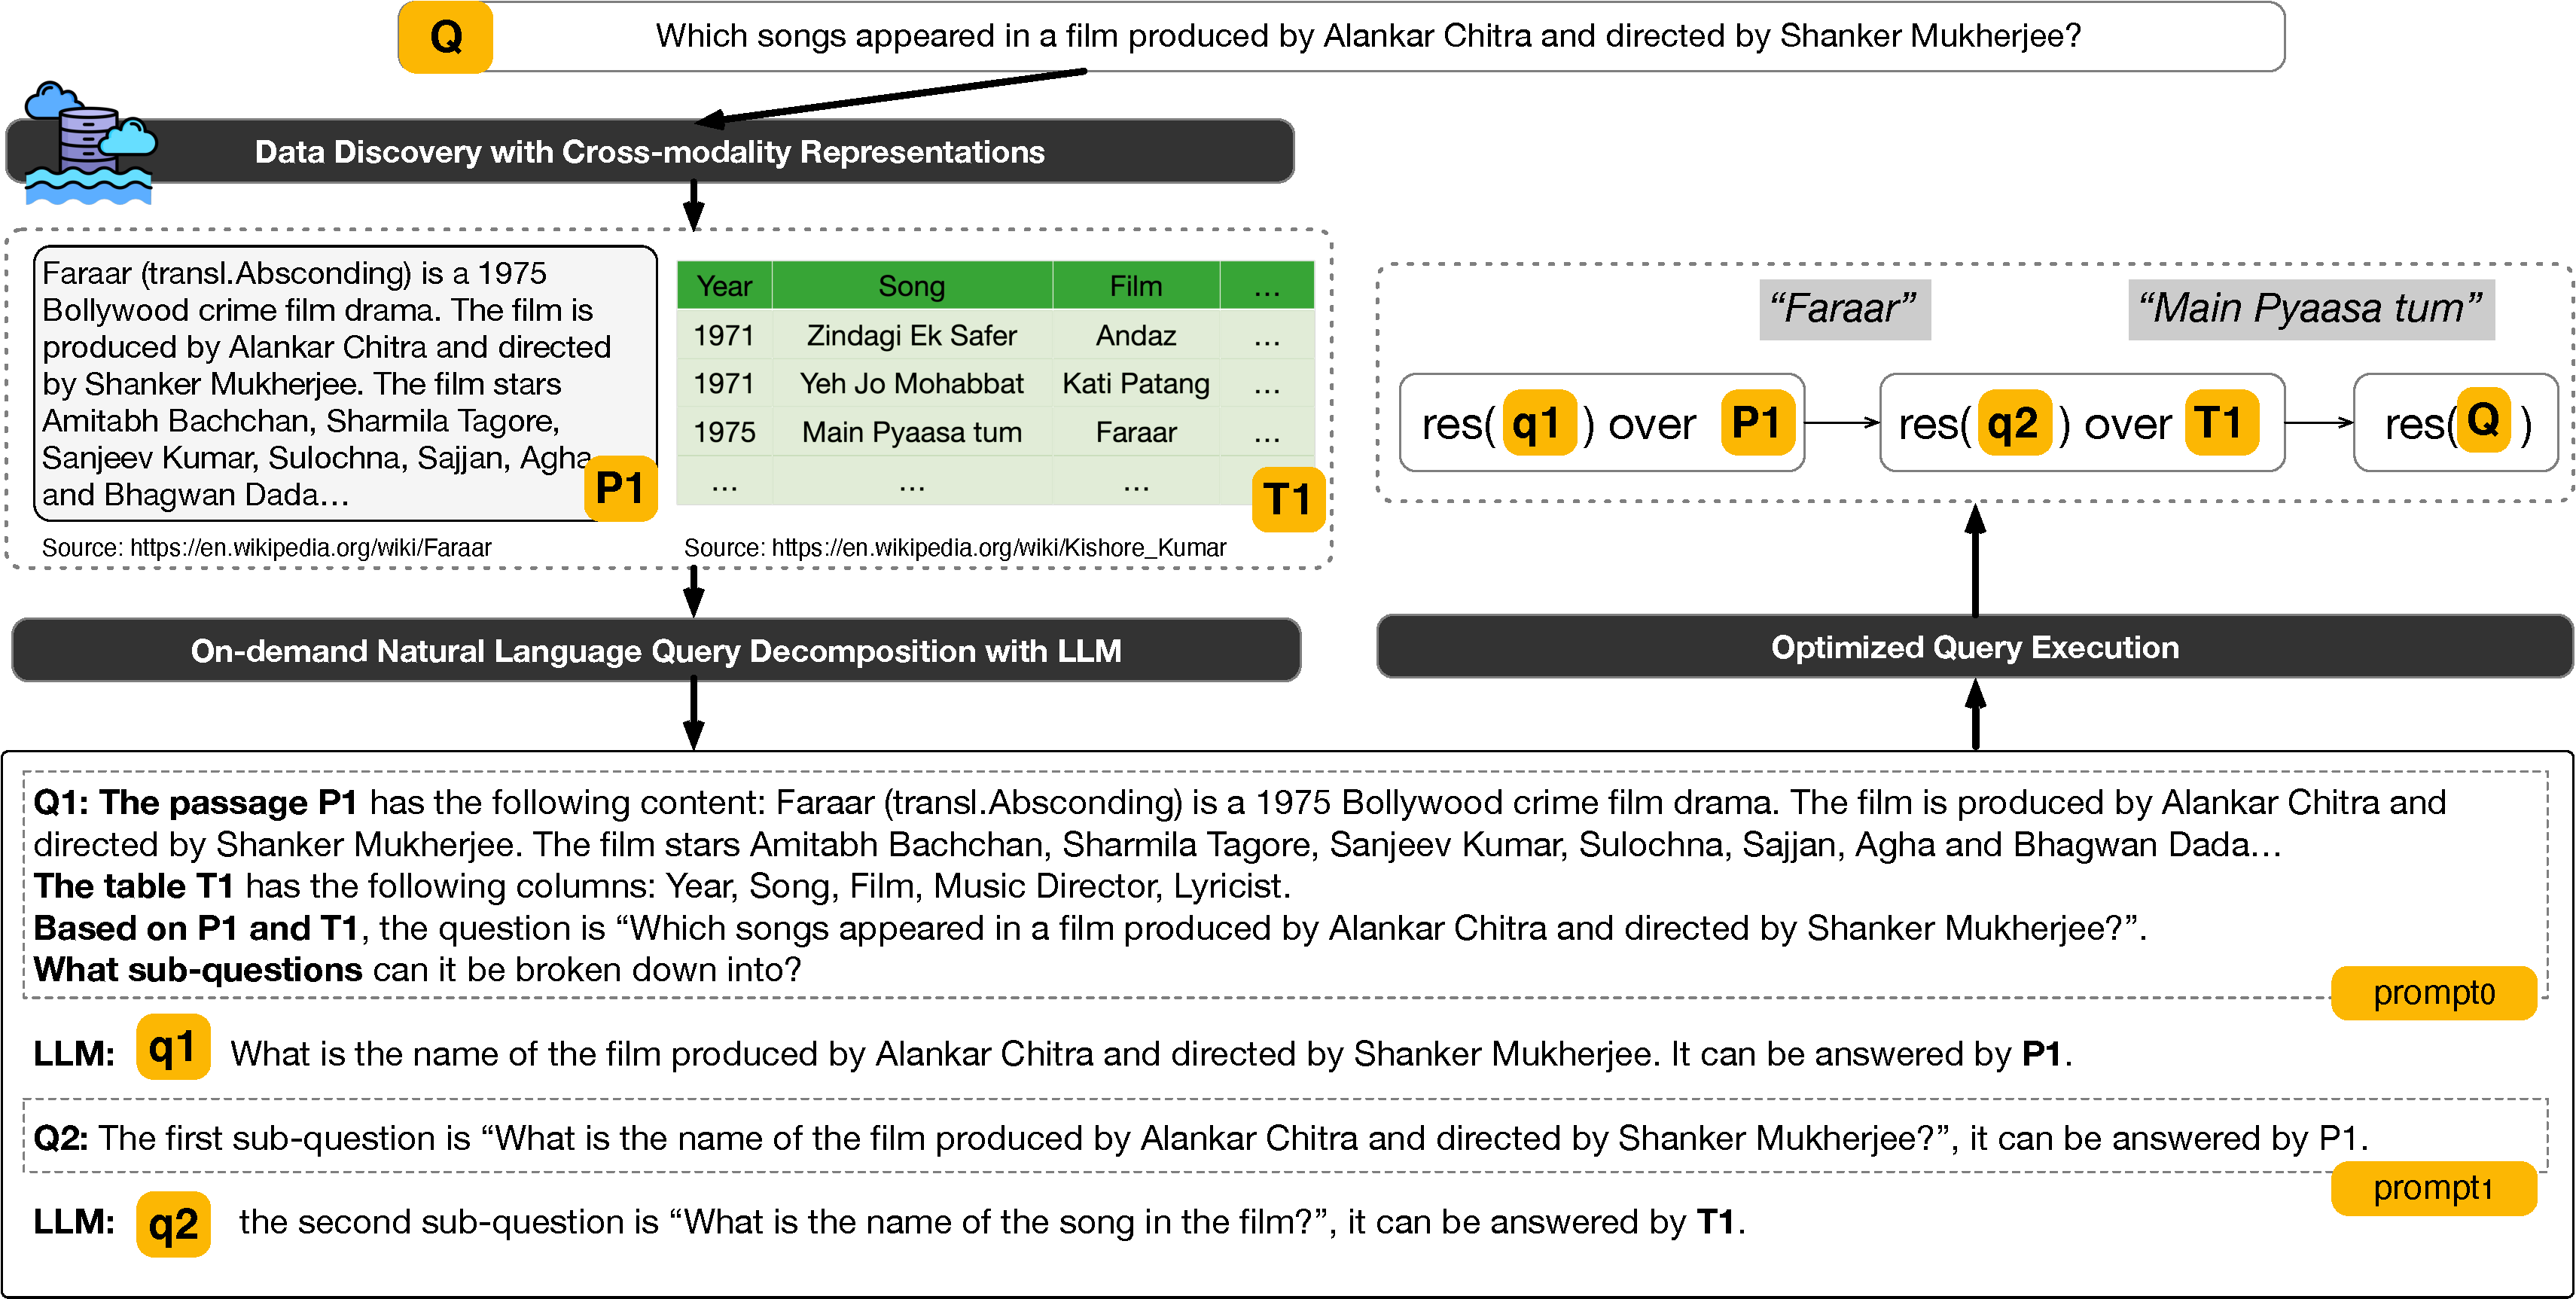
\includegraphics[width=\textwidth]{submissions/Nan2024/figs/reasoning.pdf}
\vspace{-2em}
\caption{RAG-based Reasoning in \sys}
\label{fig:reasoning}
\end{center}
\vspace{-1em}
\end{figure}


% \zzx{For image-related queries (sub-questions), we can categorize them based on the data required for retrieval: single source and multiple source. For single-source queries, such as “Who is A,” locating a single piece of data about A in the data lake is sufficient to answer the question. However, for multiple-source queries like “How many images are related to A,” multiple pieces of data related to A need to be retrieved to provide an answer.}



\subsection{Reasoning}

\stitle{Question Answering using Retrieval Augmented Generation (RAG).}
We leverage the powerful reasoning capabilities of large language models (LLMs) to address complex questions alongside relevant retrieved data sources. Using a prompt-based approach, we guide LLMs to conduct nuanced reasoning and generate coherent answers. If necessary, we can also prompt the LLM to provide detailed explanations of the reasoning, enhancing transparency and interpretability.
\sys offers NL2SQL as another way to support queries over a single table or a database.
In addition to the existing NL2SQL techniques~\cite{pasta}, \sys leverages LLMs~\cite{10.14778/3681954.3682003}, as well as the prompting techniques to convert NL questions to SQL queries, using similar ideas we introduced in question decomposition.



\stitle{Sub-Answers Aggregation.}
For complex questions, answers to each sub-question need to be combined accurately for a complete response. Using a prompt-based approach, the LLM sequentially integrates individual answers, rephrasing them into a coherent response to the original question. For instance, if the task involves summing values from sub-answers, the LLM aggregates these values directly, producing a reliable and context-aware final result.


\stitle{Reasoning Optimization.}
To ensure both efficiency and accuracy, reasoning optimization is applied to streamline execution plans and reduce response times. \sys employs a multi-objective optimizer that balances speed with precision, choosing the best approach based on retrieved data type and question complexity. For instance, if an exact result is critical and the data is highly structured, \sys prioritizes Natural Language to SQL (NL2SQL) for accuracy; otherwise, Table Question Answering (TableQA) can be used for faster, approximate answers.

% \begin{figure}[t!]
%     \vspace{-1em}
%     \centering
%     \includegraphics[width=0.8\linewidth]{submissions/Nan2024/figs/graph_reasoning.pdf}
%     \vspace{-1em}
%     \caption{VEQA Reasoning with Matching Graph}
%     \label{fig:graph_reasoning}
%     \vspace{-1em}
% \end{figure}


This optimization framework also manages cost-performance trade-offs by evaluating the computational demands of various query methods. For high-priority questions, accurate methods are selected, while non-critical evaluating may utilize quicker, approximate options. This flexible approach enables \sys to handle complex, multimodal evaluating efficiently, effectively decomposing and aggregating responses across data sources.

% \stitle{Visual-based Entity Question Answering.}
% In addition to general text, table, and image question answering, we further investigate a specific type of question: Visual-based Entity Question Answering (VEQA). As illustrated in Figure~\ref{fig:graph_reasoning}, this type of questioning focuses on entities, particularly person entities, \eg ``who is the `A' (person) in the image?'' or ``who is `A' (person) that `B' (person) are talking to?'' Due to the need for fine-grained image and name matching to accurately identify the same entity, traditional coarse-grained RAG methods are inadequate. To address this, we propose a reasoning framework based on a matching graph~\cite{zhang2024mar}. This framework operates in two key stages: matching graph construction and answer generation.



% In the matching graph construction stage, we start by initializing a seed node based on the query. For example, the input query $Q$ is associated with an image of a person, which serves as the seed node. The system then performs graph expansion by retrieving visually and semantically similar entities from the multimodal data lake. Next, in the graph optimization step, additional nodes and edges are added based on refined similarity calculations and we obtain the final matching graph.

% Based on it, we offer two methods for answer generation tailored for different scenarios. The first method, LLM + Fine-grained RAG, aggregates information from the graph and generates the answer $A1$. This approach transforms the graph's data into natural language, integrating it with the query to produce the answer. Although this method is highly adaptable, the quality of the answers relies heavily on the LLM, which may result in significant costs and delays.
% The second method, Matching-Augmented Reasoning, involves reasoning based on the graph's edges and weights. In this mothod, the system examines the relationships between the seed node and other nodes (\eg John McCain and Joe Biden), their weigh, and the frequencies, then generates the answer ($A2$) using a predefined response template. This method provides high accuracy and quick responses, but it may require specific algorithms for different types of queries.